\documentclass[
    12pt, % Font size
    openright,
    twoside, % Use both sides of the paper
    a4paper, % Paper size
    article,
    english,brazil % languages: the last one is the default of the text
]{abntex2}

\usepackage{geometry}
 \geometry{
 a4paper,
 total={170mm,257mm},
 left=20mm,
 top=20mm
 }

% Define font 
\usepackage{fourier}
\usepackage{amsmath}

% Table type
\usepackage{tabularx}

% Graphics
\usepackage{graphicx}

% accentuation support according to the compiler used
\usepackage{ifxetex}
\ifxetex
    \usepackage{fontspec}
    \defaultfontfeatures{Ligatures={TeX}}
\else
    \usepackage[utf8]{inputenc}
    \usepackage[T1]{fontenc}
\fi
% end of accentuation configuration

\usepackage{indentfirst}
\usepackage{color}
\setlength{\parskip}{0.5em}

\author{Antonio Carlos Soares Cardoso}
\title{Física - Mecânica Clássica}
\local{Brasília, DF}
\data{Maio - 2022}

%Formating section
\usepackage{titlesec}
\titleformat{\section}[hang]
{\normalfont\bfseries\filright}
{\Large\thesection.}{1ex}{\Large}
[\vspace{1ex}%
{\titlerule[2pt]}]

%Formating subsection
\titleformat{\subsection}[hang]
{\normalfont\bfseries\filright}
{\thesubsection}{1ex}{}

%Formating Table of Contents
\makeatletter
\renewcommand\tableofcontents{%
  \null\hfill\textbf{\Large\contentsname}\hfill\null\par
  \@mkboth{\MakeUppercase\contentsname}{\MakeUppercase\contentsname}%
  \@starttoc{toc}%
}
\makeatother

\begin{document}

\begin{capa}
    \center
    \ABNTEXchapterfont\Large Mecânica Clássica\\
    \vspace*{1cm}
    {\ABNTEXchapterfont\large\imprimirautor}
    \vfill
    \begin{center}
    \ABNTEXchapterfont\bfseries\LARGE\imprimirtitulo
    \end{center}
    \vfill
    \large\imprimirlocal \\
    \large\imprimirdata
    \vspace*{1cm}
\end{capa}

\tableofcontents

\newpage

\textual

\section{Mecânica Clássica}

A Mecânica Clássica corresponde à área da Física que estuda o movimento dos corpos. Para fins didáticos pode ser subdividida em:

\begin{itemize}
    \item \textbf{Cinemática} - Estuda o Movimento dos corpos em si, sem deter-se na análise de suas causas.
    \item \textbf{Dinâmica} - Analisa as causas que podem provocar movimento nos corpos.
    \item \textbf{Estática} - Analisa os corpos em equilíbrio.
\end{itemize}

De modo geral, a Mecânica Clássica pode ser utilizada na análise do movimento de corpos que não tenham velocidades comparáveis à velocidade da luz. Nesta situação, efeitos relativísticos teriam que ser considerados.

\subsection{Cinemática}

O estudo do movimento de um corpo na cinemática, em geral, corresponde à análise da posição deste ao longo de um período de observação.

Para definir uma posição é necessário estabelecer-se um referencial, a partir do qual são feitas as medidas de distância. Diz-se que um corpo está em movimento se sua distância ao referencial altera-se com o tempo. 

Tome-se como exemplo a tabela abaixo, na qual foram anotadas as posições de um veículo e seus respectivos horários. As distências foram medidas em relação ao Km 0 da rodovia. 

\begin{tabularx}{0.8\textwidth} { 
    | >{\centering\arraybackslash}X 
    | >{\centering\arraybackslash}X | }
   \hline
   \textbf{Tempo - (h)} & \textbf{Posição - (Km)} \\
   \hline
   0 & 0  \\
   \hline
   1 & 80 \\
   \hline
   2 & 180 \\
   \hline
\end{tabularx} 

Note-se que entre o início da observação e a primeira hora, o veículo percorreu 80 Km, enquanto que no intervalo entre a primeira e a segunda hora, a distância percorrida foi de 100 Km. 

À razão entre a distância percorrida e o intervalo de tempo utilizado dá-se o nome de \textbf{velocidade}. No caso descrito a medida corresponde à \textbf{velocidade média} e pode ser expressa como:

$$ v_m = \frac{\Delta S}{\Delta t} $$

Para o exemplo acima, a velocidade média na primeira hora será de 80 Km/h e do segundo 100 Km/h. Se for considerado todo o percurso e o tempo total, a velocidade média será igual a 90 Km/h. 

Note-se, portanto, que se quisermos saber mais detalhes do movimento, será necessário aferir as posições do móvel em intervalos de tempo cada vez menores. No caso limite em que o intervalo aproxime-se de zero, obter-se-á a \textbf{velocidade instantânea} do corpo. 

$$ v = \lim_{\Delta t \to 0} \frac{\Delta S}{\Delta t}$$

Tem-se, portanto, que a posição $S$ é uma função do tempo e o limite acima corresponde à derivada da função $S(t)$, logo:

$$ v = \frac{dS}{dt} $$

Quando a velocidade do corpo em análise também varia com o tempo, esta variação corresponderá à aceleração.

\textbf{Aceleração} - Corresponde à taxa de variação temporal da velocidade de um corpo, ou seja:

$$ a = \frac{dv}{dt} = \frac{d^2S}{dt^2}$$

\subsection{Aceleração constante}

Em conformidade com a definição de aceleração e para o caso específico desta ser uma constante $(a)$, obtém-se as seguintes equações descritivas do movimento:

$$ \frac{dv}{dt} = a = cte. $$
$$ \int \frac{dv}{dt} dt = \int a dt = at + C $$
$$ v(t) = v_0 + at $$

Então:

$$ \int \frac{ds}{dt} dt = \int v dt = \int (v_0 + at) dt $$
$$ S(t) = S_0 + v_0 t + \frac{a t^2}{2} $$

Expressando-se $t$ em função de $v$ e substituindo em $S(t)$:

$$t = \frac{(v - v_0)}{a}$$
$$S = S_0 + \frac{(v - v_0)}{a}(v_0 + \frac{a}{2}\frac{(v - v_0)}{a})$$

Após algumas manipulações algébricas obtém-se a equação de Torricelli. 

$$v^2 = v_0^2 + 2a(S-S_0)$$

Resumidamente, as equações para análise do movimento quando a aceleração é constante (inclusive para o caso desta ser zero) são:

\begin{equation}
    \color{blue}
    v(t) = v_0 + at
\end{equation}
\begin{equation}
    \color{blue}
    S(t) = S_0 + v_0t + \frac{at^2}{2}    
\end{equation}
\begin{equation}
    \color{blue}
    v^2 = v_0^2 + 2a(S - S_0)
\end{equation}

Todas estas grandezas são vetoriais, portanto, possuem módulo, direção e sentido. Esta característica facilita a análise dos movimentos em mais de uma dimensão (como o lançamento obliquo), à medida em que é possível fazer a decomposição do movimento.

No Sistema Internacional de Unidades (SI) as unidades de tempo e distância são: segundo (s) e metro (m). Neste Sistema a aceleração é medida em $m/s^2$.

\subsection{Exercícios}

\textbf{Um foguete sobe verticalmente, a partir do solo, com aceleração $\frac{t}{10}$ durante 30 segundos. Qual a expressão para sua velocidade e posição em funções do tempo sabendo-se que $v_0 = 0$? Esboce os gráficos da posição e velocidade e adote o solo como ponto referencial.}

\textcolor{red}{A partir da expressão da aceleração é possível obter-se a velocidade a partir de uma integração}
\textcolor{red}{
    $$a(t) = \frac{dv}{dt} = \frac{t}{10}$$
    $$\int \frac{dv}{dt} dt = \int \frac{t}{10} dt $$
    $$v(t) = \frac{t^2}{20} + C $$
}

\textcolor{red}{Pela condição de contorno $v(0) = 0$ então $C = 0$, logo:}
\textcolor{red}{
    $$v(t) = \frac{t^2}{20} $$
}

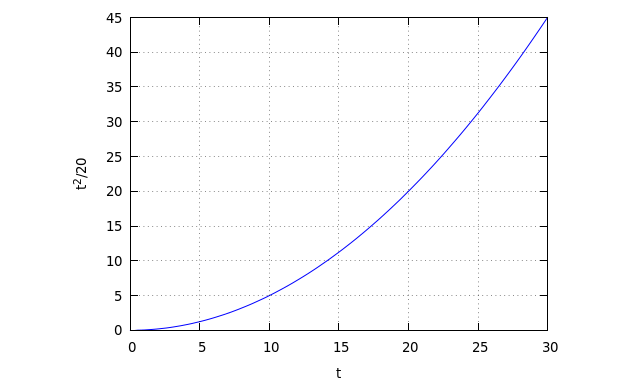
\includegraphics[width=\linewidth,height=6cm,keepaspectratio,]{./fig/exerc01-01.png}

\textcolor{red}{A partir da equação da velocidade é possível obter-se a expressão para a posição do foguete em função do tempo}

\textcolor{red}{
    $$v(t) = \frac{dS}{dt} = \frac{t^2}{20} $$
    $$\int \frac{dS}{dt} dt = \int \frac{t^2}{20} dt$$
    $$S(t) = \frac{t^3}{60} + C $$
}
\textcolor{red}{Pela condição de contorno $S(0) = 0$ então $C = 0$, logo:}
\textcolor{red}{
    $$S(t) = \frac{t^3}{60} $$
}

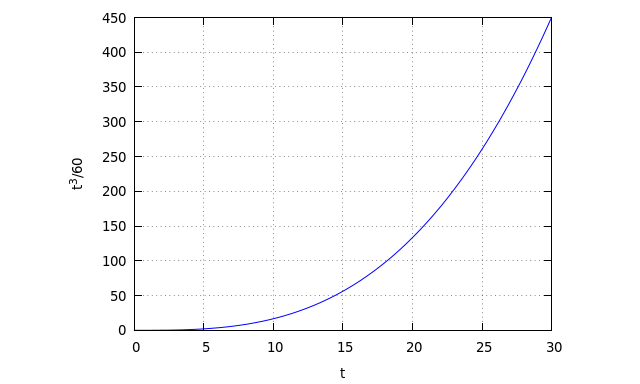
\includegraphics[width=\linewidth,height=6cm,keepaspectratio,]{./fig/exerc01-02.png}

\textbf{Um projétil é lançado obliquamente com velocidade $V$, formando um ângulo $\theta$ com a superfície horizontal. Obtenha as expressões para a altura máxima, alcance (máxima distância horizontal) e o ângulo $\theta$ que maximiza este alcance. Considere $g$ como a aceleração da gravidade.}

\textcolor{red}{O movimento pode ser decomposto em componentes vetoriais horizontal e vertical $V_x$ e $V_y$ respectivamente. No movimento horizontal não há aceleração, enquanto que no vertical atua a gravidade $g$. Desta forma, as expressões para as velocidades e as equações horárias (posição em função do tempo) são:}

\textcolor{red}{
    $$V_x = V cos(\theta)$$
    $$Vo_y = V sin(\theta)$$
}

\textcolor{red}{$Vo_y$ corresponde ao valor inicial da velocidade vertical.}

\textcolor{red}{
    $$S_x(t) = V cos(\theta) \cdot t$$
    $$S_y(t) = V sin(\theta) \cdot t - \frac{gt^2}{2}$$
}

\textcolor{blue}{\textbf{Cálculo da Altura Máxima:}}

\textcolor{red}{A Altura Máxima ($H$) ocorrerá no instante em que a derivada temporal de $S_y(t)$ for nula.}

\textcolor{red}{
    $$\frac{dS_y}{dt} = V sin(\theta) - gt = 0$$
    $$t = \frac{V sin(\theta)}{g}$$
}

\textcolor{red}{
    $$H = V sin(\theta) \cdot \frac{V sin(\theta)}{g} - \frac{g (\frac{V sin(\theta)}{g})^2}{2}$$
    $$H = \frac{V^2 sin^2(\theta)}{2g}$$
}

\textcolor{blue}{\textbf{Cálculo do Alcance ($A$):}}

\textcolor{red}{Para obter-se o alcance ($A$) é necessário identificar o tempo total de queda do projétil.}

\textcolor{red}{
    $$S_y(t) = V sin(\theta) \cdot t - \frac{gt^2}{2} = 0$$
    $$V sin(\theta) - \frac{gt}{2} = 0$$
    $$t = \frac{2V sin(\theta)}{g}$$
}

\textcolor{red}{A posição horizontal para o tempo encontrado será o alcance.}

\textcolor{red}{
    $$S_x(t) = V cos(\theta) \cdot t$$
    $$A = V cos(\theta) \cdot \frac{2V sin(\theta)}{g}$$
    $$A = \frac{2V^2 cos(\theta)sin(\theta)}{g}$$
}

\textcolor{red}{De acordo com a expressão, $A$ é função do ângulo $\theta$, portanto, o alcance máximo será quando a derivada deste em relação a $\theta$ for nula.}

\textcolor{red}{
    $$\frac{dA}{d\theta} = \frac{2V^2}{g}(-sin^2(\theta) + cos^2(\theta))$$
    $$\frac{2V^2}{g}(-sin^2(\theta) + cos^2(\theta)) = 0$$
    $$cos(\theta) = sin(\theta) \implies \theta = 45^\circ$$
}

\subsection{Dinâmica}

A Dinâmica analisa as causas do movimento. Para isto é necessário conhecer as Leis de Newton.

\end{document}